\documentclass{article}

% Language setting
% Replace `english' with e.g. `spanish' to change the document language
\usepackage[english]{babel}

% Set page size and margins
% Replace `letterpaper' with `a4paper' for UK/EU standard size
\usepackage[letterpaper,top=2cm,bottom=2cm,left=3cm,right=3cm,marginparwidth=1.75cm]{geometry}

% Useful packages
\usepackage{amsmath}
\usepackage{graphicx}
\usepackage[colorlinks=true, allcolors=blue]{hyperref}

\title{Lab 2: Device's information}
\author{Pham Quang Duong - 2540048}

\begin{document}
\maketitle

The objective of this lab is to use \texttt{numba} to retrieve information about the available GPU, including the device name, device id, core information, and memory size.

The GPU information obtained is:
\begin{itemize}
    \item Device ID: 0
    \item Device name: Tesla T4
    \item Compute Capability: 7.5
    \item Multiprocessor count: 40
    \item Total CUDA cores: $40 \times 64 = 2560$
    \item Memory Size: $14911.69$ MB
\end{itemize}

The following figure shows the output obtained from the labwork.

\begin{figure}[h]
    \centering
    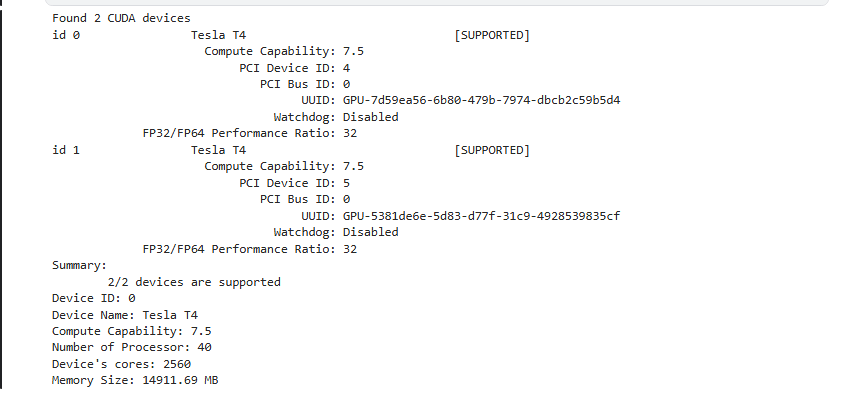
\includegraphics[width=\textwidth]{GPU_Information.png}
    \caption{GPU information obtained using \texttt{numba.cuda}.}
\end{figure}

\end{document}